\chapter{Implementation}\label{chapter:implementation}
This chapter covers the details of the implementation of a prototype regular expressions engine that takes an input file and a regular expression pattern that is transformed into efficient machine code and dynamically executed on each line of the input file using LLVM JIT Compiler. The prototype is developed using C++ and can be found on Github \footnote{\url{https://github.com/melzareix/jit-regex}}.

\section{System Architecture}
The prototype includes a regular expressions engine called \textit{ZRegex}, A Command Line Interface (CLI) application to interact with the engine, a benchmark suite, and scripts to generate the data and cases for the benchmarks. We discuss the benchmarks in detail in Chapter \ref{chapter:evaluation}. The engine is meant to be used as a sub-engine inside an RDBMS (Relational Database Management System) to provide the functionality of regular expressions matching in a fast and efficient way. The high-level system architecture of the engine is shown in Figure \ref{fig:sa}.

The inputs to the engine illustrated as yellow boxes in Figure \ref{fig:sa} are (1) a regular expression pattern to compile (needle) and (2) an input file or string to search for the pattern inside (haystack) (3) Optionally a number of configuration arguments to control the behavior of the engine that are summarized in Table \ref{tab:cliconf}. 

{\renewcommand{\arraystretch}{1.5}% for the vertical padding
\begin{table}[htpb]
\centering
\begin{adjustbox}{width=\textwidth,center=\textwidth}
\small
\begin{tabular}{|l|l|l|}
\hline
Option        & Description & Default  \\
\hline
Codegen backend & The Codegen backend to use. Possible options are {LLVM, CPP} & LLVM\\
\hline
Bytedfa & If true the DFA is utf-8 encoded otherwise it uses utf-32 & false \\
\hline
AsciiEncoding & If true disables UTF-8 handling in the generated code & false \\
\hline
\end{tabular}
\end{adjustbox}
\caption[CLI Configuration Options]{CLI Configuration Options.}\label{tab:cliconf}
\end{table}}

The engine validates the pattern, parses it and generates a parse tree. We discuss the implementation of the parser in detail in Section \ref{section:parser}. The DFA Generator checks the pattern if it is simple enough to delegate it to a more efficient matcher. The matcher uses the SIMD instruction set which we describe in detail in Section \ref{section:simdopt}.

If the pattern simplicity check fails, the DFA generator traverses the parse tree and produces a minimal DFA that can recognise the regular expression. The \textit{Codegen} module converts the DFA to efficient LLVM IR after that. The LLVM JIT Compiler compiles the IR and returns a function pointer for matching the compiled pattern against the input file.

\begin{figure}[htpb]
\centering
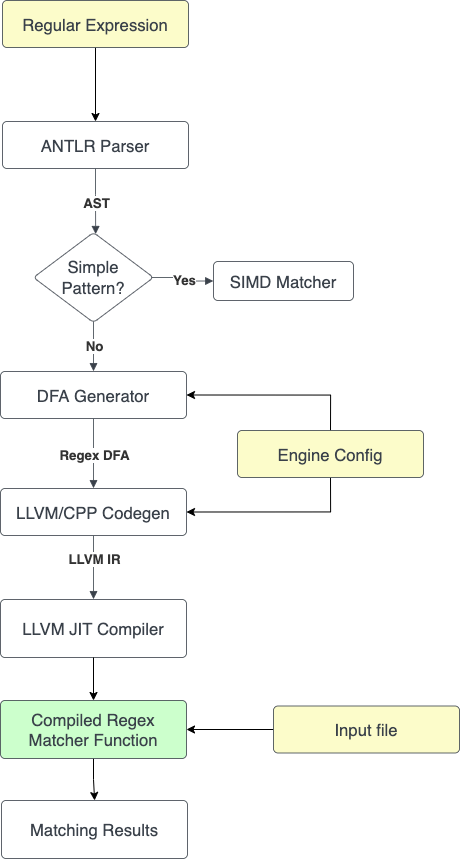
\includegraphics[width=0.65\textwidth]{imgs/sa-ext2.png}
\caption[System Architecture]{High Level System Architecture.}\label{fig:sa}
\end{figure}


% \begin{figure}[ht]
% \centering
% 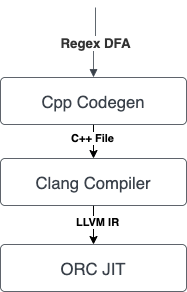
\includegraphics{imgs/sa3.png}
% \caption[C++ Code Generator]{C++ Code Generator.}\label{fig:sa3}
% \end{figure}

\section{Parser}\label{section:parser}
Initially we developed a hand-written parser for regular expressions recognition but it was (1) incredibly time consuming (2) required writing a lot of boilerplate code (3) extending the grammar required modifications to many parts of the source code. Thus, we decided to use a parser generator instead. A parser generator takes a grammar as input and generates source code that recognises the language defined by the grammar.

We experimented with many parser generators \textit{(f)lex, yacc, bison and ANTLR}. In the end we decided to use ANTLR (ANother Tool for Language Recognition) for the following reasons:

\begin{packed_enum}
    \item ANTLR allows and encourages the separation between the definition of the language from the code that handles the results, While Flex and Bison support only a grammar that contains actions that result in an ugly, monolithic and unreadable code.
    \item ANTLR supports writing the grammar in EBNF (Extended Backus–Naur Form) which makes it easier to represent the grammar, While Bison only supports BNF.
    \item ANTLR supports all unicode flavours, While (f)lex doesn't even support unicode.
\end{packed_enum}

\noindent ANTLR consists of two parts (1) a translator from the grammar to a lexer and parser in the target language (in our case C++) (2) a run-time library needed by the generated lexer and parser.

\noindent Since the engine is targeted for use inside a RDBMS we use a a SQL compliant grammar based on the grammar from Firebird Database \cite{2022Firebird}. Figure \ref{fig:zregexgrammar} shows the grammar used for the parser (Lexer rules emitted for clarity) in EBNF format. The Grammar shows the elements and rules for building regular expressions which are:

\begin{figure}[htbp]
\begin{minted}[breaklines=true,frame=lines,linenos]{antlr}
alternation: expression ('|' expression)*;

expression: element*;
element: atom quantifier?;

quantifier: '*' | '+' | '?' | '{' number (',' (number)?)? '}';
number: INT+;

atom: character | characterClass | Wildcard | '(' alternation ')';
character: regularCharacter | EscapeChar specialChar;

characterClass: '_' | '[' classMember+ ']' | '[^' classMember+ ']'

classMember: character | range | predefinedClass;
range: character '-' character;

predefinedClass: '[:' predefinedClassName ':]';
predefinedClassName: 'ALPHA'| 'UPPER'| 'LOWER'| 'DIGIT'| 'ALNUM'| 'SPACE'| 'WHITESPACE';

regularCharacter: UnicodeLetter | INT;
specialChar: '*' |  '+' |  Newline |  '?' |  '[' |  ']' |  '{' |  '}' |  '^' |  '-' |  '_' |  '|' |  '( |' |  ')' |  '%' |  '\\';

\end{minted}
\caption[Parser Grammar]{Regex SQL Grammar \cite{2022Firebird}}\label{fig:zregexgrammar}
\end{figure}

\begin{itemize}
    \item \textbf{Meta-Characters}: Special characters that denote an operator that instructs the regex engine how to match the other characters in the expression. List of supported meta-characters are defined in line 21.
    
    \item \textbf{Characters/Literals}: Actual characters that represent themselves. We support all valid Unicode as characters. Meta-characters must be escaped using the escape symbol \textbf{\char`\\} to be used as literals.
    
    \item \textbf{Wildcards}: The meta-character \textbf{\_} is used as a wildcard to match any character. To match a string of any length (even an empty string) the meta-character \textbf{\%} is used. These are equivalent to \textbf{.} and \textbf{.*} respectively in POSIX Basic Regular Expression Syntax.
    
    \item \textbf{Character Classes}: A character class is defined by a group of characters wrapped in square brackets. A character matches a class in the pattern if the character is a member of the class e.g a pattern \textbf{[abcd]} matches if the string contains \textit{any} of the characters a,b,c,d. A character class can also be negative if it starts with the \textbf{\^{}} symbol meaning it will match any character but the ones defined in the class e.g \textbf{[\^{}ab]} will match \textit{xy} but not \textit{ax}.
    
    \item \textbf{Character Ranges}: A range is defined by two characters separated by a hyphen within a class specification. A range is made up of the two endpoints and all the characters between them are defined in the class. e.g the character class \textbf{[abcd]} can be defined as an equivalent range \textbf{[a-d]}.
    
    \item \textbf{Quantifiers} A character can be followed by a quantifier that defines how many times the character can be repeated. The available quantifiers are summarized in Table \ref{tab:regexquant}.
    

\newcounter{magicrownumbers}
\newcommand\rownumber{\stepcounter{magicrownumbers}\arabic{magicrownumbers}}

{\renewcommand{\arraystretch}{1.5}% for the vertical padding
\begin{table}[H]
\centering
% \begin{adjustbox}{width=1.1\textwidth,center=\textwidth}
\small
\begin{tabular}{|l|l|l|l|}
\hline
\# & Quantifier        & Min & Max  \\
\hline
\rownumber & * & 0 & \infty\\
\hline
\rownumber & ? & 0 & 1\\
\hline
\rownumber & + & 1 & \infty\\
\hline
\rownumber & \{a, b\} & a & b \\
\hline
\rownumber & \{a\} & a & a\\
\hline
\rownumber & \{a,\} & a & \infty\\
\hline
\end{tabular}
% \end{adjustbox}
\caption[Regex Quantifiers]{Regex Quantifiers.}\label{tab:regexquant}
\end{table}}

\item \textbf{Alternations}: The meta-character \textbf{|} defines an alternation which introduces branches to the pattern e.g \textbf{[foo|bar]} matches either \textit{foo} or \textit{bar}.
\end{itemize}

% Modern Regular expression engines define some extra features which we currently don\'t support:
% \begin{itemize}
%     \item \textbf{Back-references}: 
% \end{itemize}
\section{DFA Generator}
The parser produces a parse tree that is passed to the DFA Generator module shown in Figure \ref{fig:sa2}.
This module is responsible for traversing the parse tree and applying Thompson\textquotesingle s Construction algorithm to generate an NFA that recognizes the language defined by the regular expression. The NFA is then converted to an equivalent DFA using the Power-set Construction algorithm. Several optimizations are applied to the DFA to reduce it size and possibly a DFA minimization algorithm e.g. Hopcroft\textquotesingle s algorithm is applied. 


\begin{figure}[htpb]
\centering
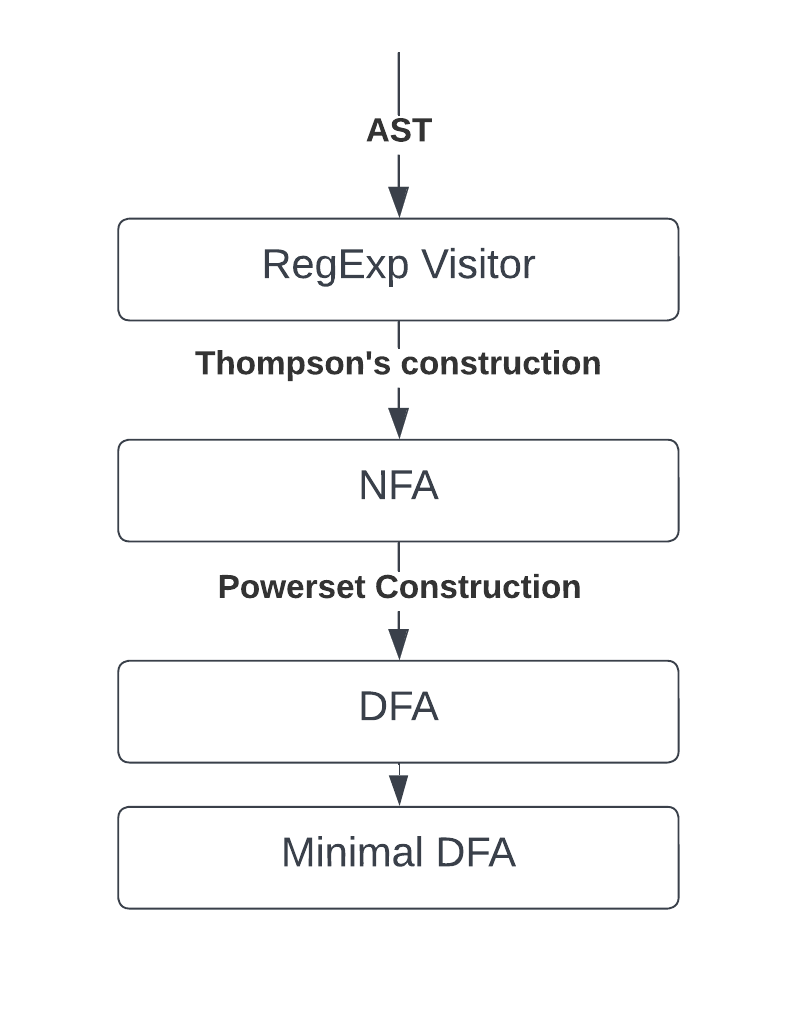
\includegraphics[width=0.45\textwidth]{imgs/sa2.png}
\caption[DFA Generator]{DFA Generator Module.}\label{fig:sa2}
\end{figure}

\subsection{Finite-Automata Representation}
Listing \ref{lst:fas} shows a simplified structure of a finite automaton which is inspired by the design of the \texttt{dk.brics.automaton}\cite{dk} Java library for finite-state automata and regular expressions.

The \texttt{\textbf{FiniteAutomaton}} class represents a generic finite automaton. It consists of two fields \texttt{\textbf{initial\_state}} pointer to the initial state of the automaton and the boolean \texttt{\textbf{deterministic}} to determine the type of the automaton \texttt{\textbf{\{NFA, DFA\}}}. Each automaton state has a unique global \texttt{\textbf{id}} field, a boolean \texttt{\textbf{accept}} to mark the state as a final accept state and a set of transitions. Each transition has a \texttt{\textbf{min}} and \texttt{\textbf{max}} fields to represent the range of input values that the transition is active for and a pointer \texttt{\textbf{to}} that represents the next state. Representing each transition as range instead of a single character simplifies the code generation phase and decreases the size of the transition table as shown in Figure \ref{fig:automatonrange}. Listing  \ref{lst:faexamplecode} shows an example how to represent the pattern \texttt{\textbf{(a|b|c)d}} using the aforementioned structures.

\begin{listing}[htpb]
\begin{minted}[breaklines=true,frame=lines,linenos]{cpp}
class FiniteAutomaton {
    public:
        bool deterministic;
        std::shared_ptr<FiniteAutomatonState> initial_state;
}

class FiniteAutomatonState {
    public:
        uint32_t id;
        bool accept;
        std::unordered_set<FiniteAutomatonTransition> transitions;
}

class FiniteAutomatonTransition {
    public:
        uint32_t min, max;
        std::shared_ptr<FiniteAutomatonState> to;
}
\end{minted}
\caption[Finite Automata Structure]{Simplified FA Structure}\label{lst:fas}
\end{listing}


\begin{listing}[htpb]
\begin{minted}[breaklines=true,frame=lines,linenos]{cpp}
    // states s0,s1,s2
    auto s0 = std::make_shared<FiniteAutomatonState>();
    auto s1 = std::make_shared<FiniteAutomatonState>();
    auto s2 = std::make_shared<FiniteAutomatonState>();
    
    // fa object with s0 as initial state
    auto fa = std::make_unique<FiniteAutomaton>(s0);
    
    // add transitions s0->s1 and s1->s2
    s0.transitions.emplace(('a', /*min*/, 'c' /*max*/, s1);
    // min = max since transition with single char
    s1.transitions.emplace('d', 'd', s2);
    
    s2.accept = true; // s2 is final state
    fa.deterministic = true; // since it is a DFA
\end{minted}
\caption[Sample Code to Create FA for pattern]{Sample Code to Create FA for pattern \textbf{(a|b|c)d}}\label{lst:faexamplecode}
\end{listing}

\begin{figure}[htpb]
\begin{subfigure}[b]{\textwidth}
\centering
\begin{tikzpicture}[->,>=stealth',shorten >=1pt,auto,node distance=3.5cm,
        scale = 1,transform shape]

  \node[state,initial] (s0) {$s0$};
  \node[state] (s1) [right of=s0] {$s1$};
  \node[state,accepting] (s2) [right of=s1] {$s2$};

  \path (s0) edge       [bend left]        node {$a$} (s1)
        (s0) edge       node {$b$} (s1)
        (s0) edge       [bend right]       node {$c$} (s1);
  \path    (s1) edge                          node {$d$} (s2);

\end{tikzpicture}
\caption{DFA with Regular Transitions}
\label{fig:automatonrangea}
\end{subfigure}
\par\bigskip
\begin{subfigure}[b]{\textwidth}
\centering
\begin{tikzpicture}[->,>=stealth',shorten >=1pt,auto,node distance=3.5cm,scale = 1,transform shape]

  \node[state,initial] (s0) {$s0$};
  \node[state] (s1) [right of=s0] {$s1$};
  \node[state,accepting] (s2) [right of=s1] {$s2$};

  \path (s0) edge              node {$[a-c]$} (s1);
  \path (s1) edge              node {$d$} (s2);
\end{tikzpicture}
\caption{Smaller DFA with Transition Ranges}
\label{fig:automatonrangeb}

\end{subfigure}
\caption{Example DFA for pattern \textbf{(a|b|c)d}.}\label{fig:automatonrange}
\end{figure}

\subsection{Regular Expression to NFA}
ANTLR generates in addition to the lexer and parser code an abstract class \texttt{\textbf{ParseTreeVisitor}} that contains methods that are called when walking the Parse Tree and implements the Visitor design pattern. Listing \ref{lst:fasvisitor} shows a snippet of the class. While walking the parse tree we visit each tree node and based on the node type and context we use Thompson's Construction algorithm explained below to generate the NFA.

\subsubsection{Literals}
% TODO: one transition
A character literal is is represented by an automaton of two states as in Figure \ref{fig:auto1}.

\begin{figure}[htpb]
\centering
\begin{tikzpicture}[->,>=stealth',shorten >=1pt,auto,node distance=3.5cm,scale = 1,transform shape]

  \node[state,initial] (s0) {$s0$};
  \node[state,accepting] (s1) [right of=s0] {$s1$};

  \path    (s0) edge                          node {$a$} (s1);

\end{tikzpicture}
\caption{Automaton to recognize the pattern \texttt{\textbf{a}}}
\label{fig:auto1}
\end{figure}


\subsubsection{Alternations}
A new state \texttt{\textbf{p}} is added with epsilon transition to the start state of each alternation. An epsilon transition from \texttt{\textbf{state0}} to  \texttt{\textbf{state1}} is equivalent to adding all transitions of state1 and marking  \texttt{\textbf{state0}} as accept if  \texttt{\textbf{state1}} was an accept state then removing  \texttt{\textbf{state1}} from the new automaton. Figure \ref{fig:auto2} shows the alternation between the two patterns \texttt{\textbf{a}} and \texttt{\textbf{x}}.

\begin{figure}[htpb]
\centering
\begin{tikzpicture}[->,>=stealth',shorten >=1pt,auto,node distance=3.5cm,scale = 1,transform shape]

  \node[state,initial] (p) {$p$};
%   \node[state] (s0) [right of=p] {$s0$};
%   \node[state] (s1) [below of=s0] {$s1$};
  \node[state,accepting] (s2) [right of=p] {$s2$};
  \node[state,accepting] (s3) [below of=s2] {$s3$};

  \path    (p) edge                          node {$a$} (s2);
  \path    (p) edge                          node {$x$} (s3);
%   \path    (s0) edge                          node {$a$} (s2);
%   \path    (s1) edge                          node {$x$} (s3);

\end{tikzpicture}
\caption{Automaton to recognize the alternation between the patterns \texttt{\textbf{a}} and \texttt{\textbf{x}}.}
\label{fig:auto2}
\end{figure}

\subsubsection{Concatenation}
The initial state of the first automaton becomes the initial state of the new NFA, the accept states of the first automaton aren\'t accept anymore and the accept states of the second automaton are the accept states of the new NFA. Figure \ref{fig:auto3} shows the concatenation between two patterns \texttt{\textbf{a}} and \texttt{\textbf{bc}}.

\begin{figure}[htpb]
\centering
\begin{tikzpicture}[->,>=stealth',shorten >=1pt,auto,node distance=3.5cm,scale = 1,transform shape]

  \node[state,initial] (s0) {$s0$};
  \node[state] (s1) [right of=s0]{$s1$};
  \node[state] (p1) [right of=s1] {$p1$};
  \node[state,accepting] (p2) [right of=p1] {$p2$};

  \path    (s0) edge                          node {$a$} (s1);
  \path    (s1) edge                          node {$b$} (p1);
  \path    (p1) edge                          node {$c$} (p2);

\end{tikzpicture}
\caption{Automaton to recognize the concatenation of the patterns \texttt{\textbf{a}} and \texttt{\textbf{bc}}.}
\label{fig:auto3}
\end{figure}

\subsubsection{Quantifiers}
\textbf{Kleene Star}: Row 1 in Table \ref{tab:regexquant} is the Kleene star \texttt{\textbf{*}} quantifier. It is an unbounded quantifier and is supported by adding a loop to the NFA. A new start state \texttt{\textbf{p}} is added with epsilon transition to the start state the automaton. Epsilon transitions from the accept states to \texttt{\textbf{p}} is added and \texttt{\textbf{p}} is marked as accept. An example for Kleene star is show in Figure \ref{fig:autoq1}.

\begin{figure}[H]
\centering
\begin{tikzpicture}[->,>=stealth',shorten >=1pt,auto,node distance=3.5cm,scale = 1,transform shape]

  \node[state,initial,accepting] (p) {$p$};
  \node[state,accepting] (s0) [right of=p]{$s0$};

  \path    (p) edge                          node {$a$} (s0);
  \path    (s0) edge [loop above] node {$a$} (s0);

\end{tikzpicture}
\caption{Automaton to recognize pattern \texttt{\textbf{a*}}.}
\label{fig:autoq1}
\end{figure}



\noindent
\textbf{Optional (Zero or one)}: Row 2 in Table \ref{tab:regexquant} is the Optional quantifier \texttt{\textbf{?}}. It is a bounded quantifier and is  equivalent to the alternation of an NFA and the empty string epsilon e.g \texttt{\textbf{a?}} is equivalent to \texttt{\textbf{a|\epsilon}}. Figure \ref{fig:autoq3} shows an example Automaton.


\begin{figure}[htpb]
\centering
\begin{tikzpicture}[->,>=stealth',shorten >=1pt,auto,node distance=3.5cm,scale = 1,transform shape]

  \node[state,initial,accepting] (p) {$p$};
  \node[state,accepting] (s0) [right of=p]{$s0$};

  \path    (p) edge node {$a$} (s0);

\end{tikzpicture}
\caption{Automaton to recognize pattern \texttt{\textbf{a?}}.}
\label{fig:autoq3}
\end{figure}

\noindent
\textbf{Plus (One or more)}: Row 3 in Table \ref{tab:regexquant} is the Plus quantifier \texttt{\textbf{+}}. It is an unbounded quantifier and is equivalent to concatenation of an NFA and Kleene star of the same NFA e.g \texttt{\textbf{a+}} is equivalent to \texttt{\textbf{aa*}}. Figure \ref{fig:autoq2} shows the example Automaton.

\begin{figure}[htpb]
\centering
\begin{tikzpicture}[->,>=stealth',shorten >=1pt,auto,node distance=3.5cm,scale = 1,transform shape]

  \node[state,initial] (s0) {$s0$};
  \node[state,accepting] (p)[right of=s0] {$p$};
  \node[state,accepting] (s1) [right of=p]{$s1$};

  \path    (s0) edge                          node {$a$} (p);
  \path    (p) edge                          node {$a$} (s1);
  \path    (s1) edge [loop above] node {$a$} (s1);

\end{tikzpicture}
\caption{Automaton to recognize pattern \texttt{\textbf{a+}}.}
\label{fig:autoq2}
\end{figure}



\noindent
\textbf{Counting}\\
Row 4 in Table \ref{tab:regexquant} is the counting quantifier. It's represented as alternation e.g \texttt{\textbf{a\{1,3\}}} is equivalent to \texttt{\textbf{a(a(a|\epsilon)|\epsilon)}} or \texttt{\textbf{a|aa|aaa}}. Figure \ref{fig:autoq4} shows the example automata.

\begin{figure}[H]
\centering
\begin{tikzpicture}[->,>=stealth',shorten >=1pt,auto,node distance=3.5cm,scale = 1,transform shape]

  \node[state,initial] (s0) {$s0$};
  \node[state,accepting] (s1) [right of=s0] {$s1$};
  \node[state,accepting] (s2) [right of=s1] {$s2$};
  \node[state,accepting] (s3) [right of=s2] {$s2$};

  \path    (s0) edge node {$a$} (s1);
  \path    (s1) edge node {$a$} (s2);
  \path    (s2) edge node {$a$} (s3);

\end{tikzpicture}
\caption{Automaton to recognize pattern \texttt{\textbf{a\{1,3\}}}.}
\label{fig:autoq4}
\end{figure}


\subsubsection{Character Classes}
\textit{Positive} Character Classes are treated the same way as alternations e.g NFA for character class \texttt{\textbf{[ax]}} is equivalent to NFA recognizing \texttt{\textbf{a|x}}. Figure \ref{fig:auto2} shows the resulting automaton.

\noindent
\textit{Negative} Character Classes are equivalent to applying \texttt{\textbf{intersection}} between the \texttt{\textbf{anyChar}} wildcard automata and automata recognizing the \texttt{\textbf{Complement}} of the character class e.g \texttt{\textbf{[\textasciicircum ax]}} is equivalent to \texttt{\textbf{$\_ \cap [ax]$}}. Figure \ref{fig:auto4} shows the result automata where transitions are encoded in hex-decimal and language of the NFA is the ASCII character-set. This is operation is costly since intersection uses the cross-product automaton construction method which requires converting NFA to DFA first and is quadratic in the number of states.

\begin{figure}[htpb]

\begin{subfigure}[b]{0.5\textwidth}
\centering
\begin{tikzpicture}[->,>=stealth',shorten >=1pt,auto,node distance=3.5cm,scale = 1,transform shape]

  \node[state,initial] (s0) {$s0$};
  \node[state,accepting] (s1) [right of=s0]{$s1$};

  \path    (s0) edge  node {$[0x0-0x7F]$} (s1);

\end{tikzpicture}
\caption{Automaton for \texttt{\textbf{anyChar}}.}
\label{fig:auto41}
\end{subfigure}
\hfill
\begin{subfigure}[b]{0.5\textwidth}
\centering
\begin{tikzpicture}[->,>=stealth',shorten >=1pt,auto,node distance=5cm,scale = 1,transform shape]

  \node[state,initial,accepting] (s0) {$s0$};
  \node[state] (s1) [right of=s0]{$s1$};

  \path    (s0) edge  node {$[0x61-0x61]$} (s1);
  \path    (s0) edge  [bend right] node {$[0x78-0x78]$} (s1);

\end{tikzpicture}
\caption{Automaton for complement of \texttt{\textbf{[ax]}}.}
\label{fig:auto42}
\end{subfigure}\\


\begin{subfigure}[b]{\textwidth}
\centering
\begin{tikzpicture}[->,>=stealth',shorten >=1pt,auto,node distance=10cm,scale = 1,transform shape]

  \node[state,initial] (s0) {$s0$};
  \node[state,accepting] (s1) [right of=s0]{$s1$};

  \path    (s0) edge [bend left] node {$[0x0-0x60]$} (s1);
  \path    (s0) edge node {$[0x62-0x77]$} (s1);
  \path    (s0) edge [bend right] node {$[0x79-0x7F]$} (s1);
\end{tikzpicture}
\caption{Automaton for Intersection between Automaton \ref{fig:auto41} and Automaton \ref{fig:auto42}}.
\label{fig:auto43}
\end{subfigure}

\caption{Automaton Construction Steps for negative character class \texttt{\textbf{[\textasciicircum ax]}}. Char \texttt{\textbf{a}} is hex \texttt{\textbf{0x61}} and Char \texttt{\textbf{x}} is \texttt{\textbf{0x78}}.}
\label{fig:auto4}
\end{figure}


\begin{listing}[htpb]
\begin{minted}[breaklines=true,frame=lines,linenos]{cpp}
class RegexVisitor : public antlr4::tree::AbstractParseTreeVisitor {
public:
  /**
   * Visit parse trees produced by RegexParser.
   */
    virtual antlrcpp::Any visitRegex(RegexContext *context)=0;
    virtual antlrcpp::Any visitAlternation(AlternationContext *context)=0;
    virtual antlrcpp::Any visitExpression(ExpressionContext *context)=0;
    virtual antlrcpp::Any visitElement(ElementContext *context)=0;
    ...
\end{minted}
\caption[RegExp ParseTree Visitor Class]{RegExp ParseTree Visitor Class}\label{lst:fasvisitor}
\end{listing}


\subsection{NFA to DFA}
After generating the NFA in the previous step, it is made deterministic using \textit{Powerset Construction} algorithm. The algorithm can transform any NFA to an equivalent deterministic automaton. However, there is one disadvantage: When the algorithm is applied to an NFA with $n$ states the resulting DFA can have an exponentially larger number of states than $2^n$ \cite{dfasize}. To overcome this problem we set an adjustable limit for the number of states the DFA can have If the algorithm exceeds it we use a fallback library to handle this regular expression.

\subsubsection{Powerset Construction}
The algorithm works by mapping associating each state in the DFA with a set of NFA states and it works as follows:
\begin{enumerate}
    \item The DFA's start state is the same as the NFA's start state, plus all states accessible via $\epsilon$-transitions.
    \item If a DFA state \texttt{\textbf{p}} corresponds to a set of NFA states \texttt{\textbf{S}}, then the transition from state p on a character \texttt{\textbf{c}} is as follows:
    \begin{enumerate}
        \item Let \texttt{\textbf{S1}} be the set of NFA states that can be reached by following a transition for character \texttt{\textbf{c}} from any of \texttt{\textbf{S}}'s states.
        \item The DFA state \texttt{\textbf{p}} transitions table row for character \texttt{\textbf{c}} is the DFA State \texttt{\textbf{q}} that corresponds to the set of states accessible via zero or more epsilon transitions from any state in \texttt{\textbf{S1}}.
    \end{enumerate}
\end{enumerate}
 

In our implementation we modify the classic algorithm as follows:
 \begin{itemize}
     \item In NFA generation we remove explicit $\epsilon$-transitions we already get them in each NFA state transition table. So we can skip the parts about $\epsilon$-transitions.
     \item Each transition we have is a range not a single character so the algorithm will not work when there are transitions with intersecting character ranges. To solve this we iterate all the transition ranges in the NFA and transform them to a sorted set of non-intersecting ranges.

 \end{itemize}
 
Figure \ref{fig:ps1} shows an example conversion NFA to DFA for pattern \texttt{\textbf{xyz|xya}}.


\begin{figure}[htpb]
\begin{subfigure}[b]{\textwidth}
\centering
\begin{tikzpicture}[->,>=stealth',shorten >=1pt,auto,node distance=2cm,scale = 1,transform shape]

  \node[state,initial] (s0) {$s0$};
  \node[state] (s1) [right of=s0] {$s1$};
  \node[state] (s2) [right of=s1] {$s2$};
  \node[state,accepting] (s3) [right of=s2] {$s3$};
  \node[state] (s4) [below of=s1] {$s4$};
  \node[state] (s5) [right of=s4] {$s5$};
  \node[state,accepting] (s6) [right of=s5] {$s6$};

  \path    (s0) edge node {$x$} (s1);
  \path    (s0) edge node {$x$} (s4);
  
  \path    (s1) edge node {$y$} (s2);
  \path    (s2) edge node {$z$} (s3);
  
  \path    (s4) edge node {$y$} (s5);
  \path    (s5) edge node {$a$} (s6);
  

\end{tikzpicture}
\caption{NFA for pattern \texttt{\textbf{xyz|xya}}.}
\label{fig:ps11}
\end{subfigure}\hfill
\par\bigskip % force a bit of vertical whitespace

\begin{subfigure}[b]{\textwidth}
\centering
\begin{tikzpicture}[->,>=stealth',auto,node distance=2cm and 3cm,scale = 1,transform shape]

  \node[state,initial] (s0) {$\{s0\}$};
  \node[state] (s1) [right of=s0] {$\{s1,s4\}$};
  \node[state] (s2) [right of=s1] {$\{s2,s5\}$};
  \node[state,accepting] (s3) [right of=s2] {$\{s3\}$};
  \node[state,accepting] (s4) [below of=s3] {$\{s6\}$};

  \path    (s0) edge node {$x$} (s1);
  \path    (s1) edge node {$y$} (s2);
  \path    (s2) edge node {$z$} (s3);
  \path    (s2) edge node {$a$} (s4);
  
\end{tikzpicture}
\caption{DFA after applying powerset construction algorithm.}
\label{fig:ps12}
\end{subfigure}

\caption{Example conversion from NFA to DFA for pattern \texttt{\textbf{xyz|xya}}.}
\label{fig:ps1}
\end{figure}

\subsection{DFA Minimization}
The objective of DFA minimization is to convert a given DFA into an equivalent DFA with the fewest possible states. There are two classes of states that can be removed or merged from the original DFA without affecting the language it accepts. Without changing the language it accepts the following types of states can be removed or combined from the original DFA:
\begin{itemize}
    \item \textbf{Dead states}: states from which no accept state is reachable. These states are removed.
    \item  \textbf{Unreachable states}: are the states that are not reachable from DFA's start state for any input. These states are removed.
    \item \textbf{Non-distinguishable states}: are those that cannot be distinguished from one another for any input. These states are merged.
\end{itemize}

Dead and Unreachable states are easily removed in $O(n + m)$ where $n$ is the number of states and $m$ is the number of transitions of the DFA. There are several algorithms that can be used to identify and merge non-distinguishable states e.g Hopcroft's algorithm \cite{Hopcroftalgo} with worst case time-complexity of $O(ns log(n))$ where $n$ is the number of states and $s$ is the size of the alphabet.

In our implementation we apply the removal of dead and unreachable states but not the merging of non-distinguishable states due to its time complexity and in our experiments it didn't have much impact on the type of patterns we are interested in.

\section{Code Generation}
The last step after generating the minimal DFA is to translate it into efficient machine code. The \texttt{\textbf{CodeGen}} Module handles the conversion of the DFA to a more efficient representation and then Just-in-time (JIT) compiling the generated code which speed up regex matching at the cost of extra compilation time before matching.

Listing \ref{lst:dfainterpreted} shows simplified code for matching using interpreted DFA. The \texttt{\textbf{traverse}} function loops through the input string and for each character tries to find the transition table entry that matches. If it does not find a matching entry it stops and returns \texttt{\textbf{false}} otherwise it continues until it either encounters an accept state and returns \texttt{\textbf{true}} or the input is finished without a match and returns \texttt{\textbf{false}}.

The problem with the interpreted code is
\begin{enumerate}
    \item It has lots of indirection and memory access for accessing the DFA state and transition table.
    \item Data is not kept in CPU registers, and registers contents are evicted regularly.
\end{enumerate}

\begin{listing}[htbp]
\inputminted[breaklines=true,frame=lines,linenos]{cpp}{code/interpretted.cpp}
\caption[Interpreted DFA Code]{Interpreted DFA Matching Code}
\label{lst:dfainterpreted}
\end{listing}

The general algorithm for code generation and execution is as follows:
\begin{enumerate}
    \item The DFA is converted to single function \texttt{\textbf{traverse}} that takes two parameters the input string and its length and returns \texttt{\textbf{true}} if the pattern matches the input or \texttt{\textbf{false}} if no match is found or the input is finished before finding a match.
    \item The function consists of several code-blocks which are:
    \begin{enumerate}
        \item Entry block for the string iterator initialization.
        \item A code-block for each DFA state that consists of first a bounds check if the input is finished in which case it returns \texttt{\textbf{false}} otherwise the next string character is loaded.
        \item After that for each transition out of the state and \texttt{\textbf{if}} condition is generated that transfers the control flow to the next DFA state or returns \texttt{\textbf{true}} if the transition goes to an accept state.
    \end{enumerate}
    \item If UTF-32 Encoding is enabled three helper functions are also added to code then loads the correct code-point from the input instead of a single character.
    \item The generated code (LLVM IR) is passed to the JIT module that compiles it and then returns a function pointer to the traverse function. 
    
\end{enumerate}

\subsubsection{C++ CodeGen}
Listing \ref{lst:cppex} shows the C++ code generated for pattern \texttt{\textbf{[a-z][0-9]}}. The generated code unrolls the DFA matching loop and for each state, its transitions are also unrolled and can be treated as constant as well eliminating any memory access for the DFA, this representation in turn enables the compiler to eliminate a lot of indirection and dead code. In our implementation, we support C++ and LLVM IR code generation.

For C++ backend before the last step in the code-generation algorithm we use the LLVM \texttt{\textbf{clang}} compiler to emit Optimized LLVM IR before passing it to the JIT module that compiles it and returns a function pointer to the traverse function. 

\begin{listing}[htbp]
\inputminted[breaklines,frame=lines,linenos]{cpp}{code/ex.cpp}
\caption{Generated C++ Code for pattern \texttt{\textbf{[a-z][0-9]}}.}
\label{lst:cppex}
\end{listing}

Generating High Level code C++ code is easy to implement and debug but there are some disadvantages to this approach (1) The optimizing cpp compiler is slow compared to the LLVM Compiler. (2) Slow disk access is needed as the generated code must first be written to the disk since \texttt{\textbf{clang}} doesn't support compiling an in-memory string buffer. Therefore, The JIT Module has to read the LLVM IR from disk before being JITed which adds extra latency. For these reasons most of the code-generation work focused on the LLVM backend.


\subsubsection{LLVM CodeGen}
The \texttt{\textbf{CodeGen}} module generates code for the LLVM backend that is similar in structure to the code generated for C++ and follows the same general algorithm outlined above. However, it directly emits LLVM IR and thus faster to JIT and optimize. LLVM tool-chain provides an excellent C++ API \cite{llvmapi} to help generate and validate the IR.

Lets walk-through an example of how we go from a DFA representation to LLVM IR and how we also use the LLVM tool-chain to optimize the generated code and JIT the code. Figure \ref{fig:dfacodegenex} shows the DFA for pattern \texttt{\textbf{[a-z][0-9]}} that we will use an example. The DFA consists of three states and two transitions.

\begin{figure}[H]
\centering
\begin{tikzpicture}[->,>=stealth',shorten >=1pt,auto,node distance=2.5cm,scale = 1,transform shape]

  \node[state,initial] (s0) {$s4$};
  \node[state] (s1) [right of=s1]{$s5$};
  \node[state,accepting] (s2) [right of=s1]{$s7$};

  \path    (s0) edge                          node {$[a-z]$} (s1);
  \path    (s1) edge                          node {$[0-9]$} (s2);

\end{tikzpicture}
\caption{DFA to recognize pattern \texttt{\textbf{[a-z][0-9]}}.}
\label{fig:dfacodegenex}
\end{figure}

Table \ref{tab:llvminst} lists the LLVM IR instructions and their meaning needed to understand the code generated. Listing \ref{lst:llvmex} shows the complete code generated for the pattern. Lines 1 defines the \texttt{\textbf{traverse}} function and its parameters an unsigned char pointer which is the input text and the length of the input text.

Lines (2-5) describe the entry block in which the \texttt{\textbf{idx}} variable used to traverse the input text is defined and initialized to zero. After that an unconditional jump to initial state to start the matching process.

Lines (6-8) define the initial state block and the we do a bounds check if the current $idx >= n$. Line 9 is a conditional jump based on the result of the comparison before if the comparison is true it means the input is finished without a match in which case we go to \texttt{\textbf{bounds\_then}} block and return \texttt{\textbf{false}}.

If the bounds check is \texttt{\textbf{false}}, we jump to block \texttt{\textbf{bonds\_cont}} Lines (12-20) where we first load the next character from the input text, increment the idx variable and then check the value of the character if it is in the range $[a - z]$. If the comparison succeeds we jump to the next state block \texttt{\textbf{s5}}. Otherwise, we jump to the block \texttt{\textbf{s4\_nt}} and return \texttt{\textbf{false}} as no match is found.

Lines (23-41) repeat the same process but for the second state and the check is for the range $[0-9]$. The only difference is after matching that range we jump to block \texttt{\textbf{s7}} that returns \texttt{\textbf{true}} and indicating a match is found. Figure \ref{fig:annocfg} shows an annotated Control Flow Graph (CFG) of the generated code.

The next step after generating the LLVM IR, The LLVM optimizer is used to validate and optimize the IR. The number and type of optimization passes applied are configurable via the optimization level configuration option.

The LLVM code generator uses this optimization level to determine which optimization passes it should apply during the generation of the machine code. Each optimization level applies different optimizations to the code to aim either for speed or size of the code. Table \ref{tab:optlevels} shows the default optimization levels shipped with LLVM. By default we apply the \textbf{-O2} optimization level which is a moderate level of optimization that enables most optimizations.

{\renewcommand{\arraystretch}{1.1}% for the vertical padding
\begin{table}[H]
\centering
\small
\begin{tabularx}{\textwidth}{|l|X|}
\hline
Level        & Description  \\
\hline
\textbf{-O0} & Applies no optimizations. It compiles the fastest and generates the most debuggable code.\\
\hline
\textbf{-O2} & Is a moderate level of optimization that enables most optimizations.\\
\hline
\textbf{-O1} & Is a middle ground between -O0 and -O2.\\
\hline
\textbf{-Os} & Enables -O2 optimizations in addition to extra optimizations to reduce code size..\\
\hline
\textbf{-Oz} & Applies more optimizations to reduce code size than -Os.\\
\hline
\textbf{-O3} & Enables more optimizations than -O2 that may take longer to complete or may result in large code size (in an attempt to make the program run faster).\\
\hline
\end{tabularx}
\caption[LLVM Optimization Levels]{LLVM Optimization Levels.}\label{tab:optlevels}
\end{table}}

Applying the LLVM optimizer with Level \textbf{-O2} to the code generated yields the LLVM IR in Listing \ref{lst:llvmexs}. We notice the code size was halved from 42 to 21 lines of code. The number of code blocks was also halved and common blocks were merged into the \texttt{\textbf{common.ret}} block. This demonstrates how powerful is the LLVM optimizing compiler.

The last step after the optimization is passing the optimized IR to the JIT compiler that compiles it and
then returns a function pointer to the traverse function that is used for matching.

{\renewcommand{\arraystretch}{1.5}% for the vertical padding
\begin{table}[H]
\centering
\small
\begin{tabularx}{\textwidth}{|l|X|}
\hline
Instruction        & Description  \\
\hline
\textbf{\%reg} & A (Static Single Assignment) SSA register named \texttt{\textbf{reg}}.\\
\hline
\textbf{alloca} & Allocate a variable on the stack.\\
\hline
\textbf{getelementptr} & Get the address of a subelement of an aggregate data structure (e.g Arrays).\\
\hline
\textbf{load} & Load data from memory.\\
\hline
\textbf{store} & Write data to memory.\\
\hline
\textbf{br} & Branch to a different basic block in the current function which can be a conditional or unconditional branch. \\
\hline
\textbf{phi} & Implements the $\phi$ node in the SSA graph representing the function.\\
\hline
\textbf{and} & Performs a bitwise logical and.\\
\hline
\textbf{ret} & Returns control flow (and optionally a value) from a function back to the caller.\\
\hline
\textbf{icmp} &
Returns a boolean value or a vector of boolean values based on comparison of its integer operands.The first operand is the condition code indicating the kind of comparison to perform. Subset of possible condition codes are:\newline
\textbf{eq}: equal\newline
\textbf{ne}: not equal\newline
\textbf{ugt}: unsigned greater than\newline
\textbf{uge}: unsigned greater or equal\newline
\textbf{ult}: unsigned less than\newline
\textbf{ule}: unsigned less or equal\newline
\\
\hline
\end{tabularx}
\caption[LLVM Instructions]{LLVM Instructions.}\label{tab:llvminst}
\end{table}}


% \begin{adjustbox}{width=\textwidth}
\begin{figure}[htbp]
    \makebox[\textwidth][c]{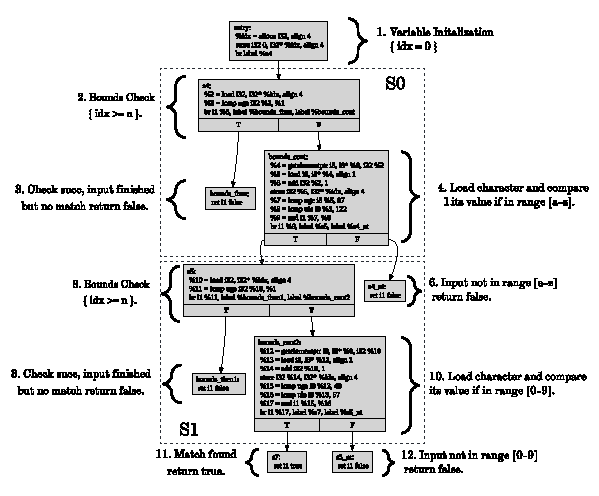
\includegraphics[width=1.42\textwidth]{code/cfga3.pdf}}%
    \caption{Annotated CFG for Generated LLVM Code for pattern \texttt{\textbf{[a-z][0-9]}} before LLVM optimizations.}
    \label{fig:annocfg}
\end{figure}
% \end{adjustbox}


\begin{longlisting}
\inputminted[breaklines=true,frame=lines,linenos]{llvm}{code/irbefore.ll}
\caption{Generated LLVM Code for pattern \texttt{\textbf{[a-z][0-9]}} before LLVM optimizations.}
\label{lst:llvmex}
\end{longlisting}


\begin{listing}[H]
\inputminted[breaklines=true,frame=lines,linenos]{llvm}{code/irafter.ll}
\caption{Generated LLVM Code for pattern \texttt{\textbf{[a-z][0-9]}} after LLVM optimizations.}
\label{lst:llvmexs}
\end{listing}

\section{Unicode}
Unicode is a standard that was created specifically to encode all of the characters in all of the world's writing systems. All modern database engines support Unicode characters and users expect some kind Unicode support. Therefore, The addition of basic Unicode support to our prototype is a must-have feature. Also since Unicode is a large character set adding Unicode support helps in testing how well our prototype scales as regular expression engines that are only adapted to handle small character sets will typically not scale well.

The Unicode Consortium has published guidelines \cite{unicodeguideline} on how regular expression engines can support Unicode. The guidelines specify three levels of Unicode support: Basic, Extended and Tailored.

Unicode level 1 support (Basic Unicode Support) defines the guidelines for minimal level for useful Unicode support. The results of regular expression matching at this level are not country or language dependent. To accomplish full Unicode processing at this level, the user of the regular expression engine would need to define more complicated regular expressions. To claim conformance with the first level of support a regular expression engine must support:

\begin{enumerate}
    \item \textbf{Hex Notation}: An implementation must provide a means for expressing any Unicode code point (from U+0000 to U+10FFFF) using the hexadecimal code point encoding to meet this criteria.
    \item \textbf{Properties}: Unicode properties provide a convenient way to construct character classes of groups of code points specified by Unicode. E.g. Unicode general category property that allows the user to express a category in a regular expression, such as "upper case letter" which encompasses all characters categorized as upper case letters in all of the world's writing systems.
    \item \textbf{Subtraction and Intersection}: An implementation must provide mechanisms for the union, intersection, and set-difference of sets of characters within regular expression character class expressions.
    \item \textbf{Simple Word Boundaries}: An engine supporting the test for word boundaries e.g the pattern \textbf{\textbackslash b} must be extended to include characters with the alphabetic property, characters from the Unicode decimal general category, zero width joiners, or zero width non-joiners.
    \item \textbf{Simple Loose Matches}: An engine supporting case-less matching must be extended to include at the very least the simple, default Unicode case-insensitive matching. Also if it supports case conversions, then it shall provide at least the simple, default Unicode case folding.
    \item \textbf{Line Boundaries}: A regular expression engine that supports line boundaries must support CRLF, LF, CR, NEL (U+0085), PARAGRAPH SEPARATOR (U+2029) and LINE SEPARATOR (U+2028).
    \item \textbf{Code Points}: A key requirement is that Unicode text be semantically interpreted by code point rather than code unit.
\end{enumerate}

Unicode level 2 support for regular expression engines is referred to as Unicode extended support. The criteria for Unicode level 2 support are requirements put in place to meet user expectations for Unicode character sequences. The major needs for this level of support are support for canonical equivalence, extended grapheme clusters, and improved word boundary detection.

Unicode level 3 defines the specifications for tailored regular expression support. A regular expression engine can be tailored for a given area and utilized by specific groups of end users.

In our prototype, We did not aim for a complete Unicode Level 1 support due to time constraints. We implemented only requirement seven \textbf{Code Points} that is that the Unicode text is interpreted semantically by code point, not code units. Adding support for requirements (1-3) is an easy task and would require mostly changes to the parser grammar. There is little to no support for either Level 2 or Level 3. Most of this is due to the features being either complex/difficult to develop or, at the very least, extremely difficult to implement without losing performance.

In our prototype, We support two modes Unicode modes for matching: UTF-8 and UTF-32. We assume for both modes that both the pattern and input string are UTF-8 encoded (which includes ASCII).

\subsection{UTF-32}
We implemented this as the first step towards handling Unicode in our prototype. 
In the UTF-32 mode the DFA generated matches full code-points and the logic for character decoding is handled outside the DFA by helper methods, effectively making the alphabet of the DFA is the full Unicode range \texttt{\textbf{0x000000-0x1FFFFF}}. Figure \ref{fig:utf32exdfa} shows the an example DFA to match the sterling character \texttt{\textsterling}.

\begin{figure}[H]
\centering
\usetikzlibrary{fit}
\begin{tikzpicture}[->,>=stealth',shorten >=1pt,auto,node distance=2.5cm,scale = 1,transform shape]

  \node[state,initial] (s0) {$s0$};
  \node[state,accepting] (s1) [right of=s1]{$s1$};

  \path    (s0) edge                          node {$0x000000A3$} (s1);

\end{tikzpicture}
\caption{DFA to recognize pattern \texttt{\textsterling}.}
\label{fig:utf32exdfa}
\end{figure}

\noindent To handle the character decoding a new function \texttt{\textbf{nextByte}} is added in the  code generation step as shown in Listing \ref{lst:utf32nextbyte}. In this function the UTF-8 string is passed and the number of bytes of the code-point are determined then using the other helper function \texttt{\textbf{readMultiByte}} the complete codepoint is read and returned and we can continue the dfa matching in line \texttt{\textbf{18}}.

While UTF-32 is easy to implement and makes the DFA generation step easier and the smaller, it is space inefficient since in DFA generation we have to store each transition as 32-bit Integer and the repeated function calls and logic for UTF-8 decoding then UTF-32 encoding is costly and impacts the performance. 

\begin{listing}[htbp]
\inputminted[breaklines=true,frame=lines,linenos]{cpp}{code/utf32.cpp}
\caption[Code generated for handling Recognizing UTF-32 pattern]{Code generated for handling Recognizing UTF-32 pattern.}
\label{lst:utf32nextbyte}
\end{listing}

\subsection{UTF-8}
The default mode of operation for the engine. To support UTF-8 the engine embeds the UTF-8 decoding inside the DFA. In this mode the engine treats the input pattern is a valid UTF-8 encoded string. The DFA generation module generates a Byte DFA that is the alphabet of the DFA is $[0x0 - 0xFF]$ and to recognize a code-point the number of UTF-8 bytes to represent it are determined and then code-point is then split into a sequence of valid UTF-8 bytes.

\begin{figure}[htbp]
\centering
\begin{adjustbox}{width=1.1\textwidth,center=\textwidth}
\begin{tikzpicture}[->,>=stealth',shorten >=1pt,auto,node distance=2.5cm,scale = 1,transform shape]

  \node[state,initial] (s0) {$s0$};
  \node[state] (s1)[right of=s0] {$s1$};
  \node[state] (s2) [right of=s1]{$s2$};
  \node[state] (s3) [right of=s2]{$s3$};
  \node[state,accepting] (s4) [right of=s3]{$s4$};
  \node[draw,dotted,fit=(s2) (s3) (s4)] {};

  \path    (s0) edge                          node [scale=0.7] {$0x39$} (s1);
  \path    (s1) edge                          node [scale=0.7] {$0x20$} (s2);
  \path    (s2) edge                          node [scale=0.7] {$0xC2$} (s3);
  \path    (s3) edge                          node [scale=0.7] {$0xA3$} (s4);

\end{tikzpicture}
\end{adjustbox}
\caption{DFA to recognize pattern \texttt{9\textvisiblespace \textsterling}.}
\label{fig:utf8exdfa}
\end{figure}

\noindent For example to generate a DFA the recognizes the pattern ``\texttt{9\textvisiblespace \textsterling}" that matches the digit 9 followed by a space character then a sterling pound character which correspond to the following Unicode code-points sequence \texttt{\textbf{\textbackslash u0039\textbackslash u0020\textbackslash u00A3}}. The engine first determines that it needs 1 byte for the first two code-points and two bytes for the sterling character. Figure \ref{fig:utf8exdfa} shows the resulting DFA.

\subsubsection{Byte Ranges Transformation}

Generating byte DFA with with embedded UTF-8 decoding raises an issue with converting Unicode code-points to UTF-8 byte ranges. To demonstrate the issue lets say we want to match any Cyrillic character we can do so with the following pattern \texttt{\textbf{[\textbackslash u0400-\textbackslash u04FF]}}.  The set of allowed bytes for this range can be expressed as a sequence of byte ranges: $\langle0xD0-0xD3\rangle \langle0x80-0xBF\rangle$. We can achieve this by simply encoding the boundaries \texttt{\textbf{\textbackslash u0400}} is encoded as $\langle0xD0 \; 0x80\rangle$ and \texttt{\textbf{\textbackslash u04FF}} is encoded as $\langle0xD3 \; 0xBF\rangle$ then we can create ranges from each corresponding pair of bytes: $D0 \rightarrow 0xD3$ and $0xD3 \rightarrow 0xBF$.

Now lets try to extend the range to include Cyrillic Supplementary characters to the range. The pattern becomes \texttt{\textbf{[\textbackslash u0400-\textbackslash u052F]}}. Applying the same algorithm above \texttt{\textbf{[\textbackslash u052F}} is encoded as $\langle0xD4 \; 0xAF\rangle$ and we get the following sequence of byte ranges: $\langle0xD0-0xD4\rangle \langle0x80-0xAF\rangle$. However, this range is not correct because this range doesn't capture many characters, for example, \texttt{\textbf{\textbackslash u04FF}} as its last byte, $0xBF$ isn't in the range $\langle0x80-0xAF\rangle$. Instead we would need two sequences of byte ranges:

\begin{figure}[H]
\centering
$\langle0xD0-0xD3\rangle \langle0x80-0xBF\rangle$\\
$\langle0xD4\rangle \langle0x80-0xAF\rangle$
\end{figure}


To overcome this issue, We adapted the algorithm for solving this problem by \citet{utf8-ranges} for the rust regex crate.
Applying the correct algorithm, Figure \ref{fig:dfabmp} shows the resulting DFA for the character class for for the basic multilingual plane (BMP) \texttt{\textbf{[\textbackslash u{0000}-\textbackslash u{FFFF}]}} which is obtained by the partitioning the range to the following sequences of byte ranges:

\begin{figure}[H]
\centering
$\langle0x0-0x7F\rangle$\\
$\langle0xC2-0xDF\rangle \langle0x80-0xBF\rangle$\\
$\langle0xE0\rangle \langle0xA0-0xBF\rangle \langle0x80-0xBF\rangle$\\
$\langle0xE1-0xEC\rangle \langle0x80-0xBF\rangle \langle0x80-0xBF\rangle$\\
$\langle0xED\rangle \langle0x80-0x9F\rangle \langle0x80-0xBF\rangle$\\
$\langle0xEE-0xEF\rangle \langle0x80-0xBF\rangle \langle0x80-0xBF\rangle$
\end{figure}

\begin{figure}[htbp]
\centering
\begin{adjustbox}{width=0.8\textwidth,center=\textwidth}
\begin{tikzpicture}[->,>=stealth',shorten >=1pt,auto,node distance=3cm and 1.5cm,scale = 1,transform shape]

  \node[state,initial] (s0) {$s0$};
  \node[state] (s3) [right of=s0]{$s3$};
  \node[state] (s2) [above of=s3]{$s2$};
  \node[state] (s1) [above of=s2]{$s1$};
  \node[state] (s4) [below of=s3]{$s4$};
  \node[state] (s5) [below of=s4]{$s5$};
  \node[state,accepting] (s6) [below of=s5]{$s6$};

  \node[state] (s7) [right of=s1]{$s7$};
  \node[state] (s9) [right of=s3]{$s9$};

  \node[state] (s10) [right of=s4]{$s10$};
  \node[state,accepting] (s8) [right of=s9]{$s8$};

  \path    (s0) edge   [bend left]            node [scale=0.85,sloped] {$0xee-0xef$} (s1);
  \path    (s0) edge   [midway,align=left]         node [scale=0.8,sloped] {$0xe1-0xec$} (s2);
  \path    (s0) edge                          node [scale=0.85,sloped] {$0xed$} (s3);
  \path    (s0) edge  [bend right=20]         node [scale=0.85,sloped] {$0xe0$} (s4);
  \path    (s0) edge  [bend right=20]         node [scale=0.85,sloped] {$0xc2-0xdf$} (s5);
  \path    (s0) edge  [bend right]            node [scale=0.85,sloped] {$0x0-0x7f$} (s6);

  \path    (s1) edge                          node [scale=0.85] {$0x80-0xbf$} (s7);
  \path    (s2) edge                          node [scale=0.85,sloped] {$0x80-0xbf$} (s7);

  \path    (s7) edge [bend left]              node [scale=0.85,sloped] {$0x80-0xbf$} (s8);
  \path    (s3) edge                          node [scale=0.85] {$0x80-0x9f$} (s9);
  \path    (s9) edge                          node [scale=0.85] {$0x80-0xbf$} (s8);
  \path    (s4) edge                          node [scale=0.85] {$0xa0-0xbf$} (s10);
  \path    (s10) edge [bend right=10]                        node [scale=0.85,sloped,above] {$0x80-0xbf$} (s8);
  \path    (s5) edge [bend right=40]             node [scale=0.85,sloped] {$0x80-0xbf$} (s8);


\end{tikzpicture}
\end{adjustbox}
\caption{DFA to decode valid UTF-8 code-point for BMP range \texttt{\textbf{[\textbackslash u0000-\textbackslash uFFFF]}}.}
\label{fig:dfabmp}
\end{figure}

\section{Literal Optimizations}\label{section:simdopt}
Searching for a pattern that consists only of string literals e.g \texttt{\textbf{foobar}} is a common use-case for regular expressions matching in databases. A fast and smart regular expression engine can detect these patterns and optimize the search algorithm for them. On modern CPUs, the key to optimize the search for literals is how fast we can identify a candidate for a match. That is the reason we use Single Instruction Multiple Data (SIMD) instructions when we detect a literal. SIMD instructions can examine up to sixty-four bytes in a single loop iteration which makes it very fast.  

In our implementation we detect these simple literal patterns e.g \texttt{\textbf{.*foobar.*}} and apply one of the two algorithms explained below based on the size of the pattern.

\subsection{EPSM Algorithm}
Exact Packed String Matching (EPSM) \cite{epsm} is a string matching algorithm that makes use of bit-parallelism by packing several characters into a bit-word and partitioning string S into chunks $S_i$. A packed pattern bit-word is compared to these bit-word-sized chunks. To compare text chunks with the pattern, shift and bitwise-and operations are performed. The algorithm is based on four different search procedures that are applied based on the pattern length. In our implementation, we use this algorithm only for short patterns $(m <= 16)$ as its performance degrades as the length of the patterns increase. Under these limitations, EPSM is very fast and runs in O(n). The asymptotic run-time for the general case is $O(n ∗ m)$.

%  The main idea of the EPSMa algorithm is marking the positions of the pattern’s symbols on the investigated text chunk. 
The pseudo-code of the EPSMa algorithm is shown in Algorithm \ref{alg:espma}. The algorithm starts by a processing phase (lines 3-8) on the prefix of the pattern of length $m_i = min(m, \alpha/2)$ where $\alpha$ is the number of characters of the alphabet that fit in a single word e.g for 128-bit registers and $\gamma$ the number of bits per character = 8, $\alpha = 16$. If $m = m'$ the algorithms pre-processes and searches the whole pattern. Otherwise, the algorithm acts as a filter that searches for the occurrences of the prefix of length $m'$ then naively checking the whole occurrence of the pattern if an occurrence of the prefix is found. In the processing phase, the algorithm  constructs an array $B$ of $m'$ strings each of length $\alpha$. The $i$-th string in array $B$ consists of $\alpha$ copies of the character $p_i$.

For the searching phase we define the word-size compare instruction (\texttt{\textbf{wscmp}}) that compares its two w-bit sized inputs where $w$ is the number of bits in a computer word  handled as a block of $\alpha$ characters. Figure \ref{fig:wscmpex} shows an example application of wscmp(A,B). This instruction is equivalent to the following specialized SIMD instructions:

\begin{figure}[H]
\centering
\begin{cminted}{c}
h = mm_cmpeq_epi8(a, b)
r = mm_movemask_epi8(h)
\end{cminted}
\end{figure}

\begin{figure}[htbp]
\centering
\begin{bytefield}{16}
\bitheader{0,4,8,12,15} \\
\begin{leftwordgroup}{A:}
\bitbox{4}{\textbf{0011}} & \bitbox{4}{0111} & \bitbox{4}{\textbf{1011}} & \bitbox{4}{0000}
\end{leftwordgroup} \\
\end{bytefield}

\begin{bytefield}{16}
\bitheader{0,4,8,12,15} \\
\begin{leftwordgroup}{B: }
\bitbox{4}{\textbf{0011}} & \bitbox{4}{1011} & \bitbox{4}{\textbf{1011}} & \bitbox{4}{1111}
\end{leftwordgroup} \\
\end{bytefield}

\begin{bytefield}[bitwidth=3em]{4}
\bitheader{0-3} \\
\begin{leftwordgroup}{R:}
\bitbox{1}{1} & \bitbox{1}{0} & \bitbox{1}{1} & \bitbox{1}{0}
\end{leftwordgroup} \\
\end{bytefield}
    \caption{Example for \texttt{\textbf{wscmp(a,b)}} where $\alpha = 4$, $\gamma=4$ and $w = 16$.}
    \label{fig:wscmpex}
\end{figure}


The searching phase (lines 9-23) processes the text $t$ in blocks of $\alpha$ characters. Therefore, Lets define  $N = \frac{n}{\alpha} - 1$ and the string $t$ of length $n$ as $T=T_0 T_1...T_N$. The instruction \texttt{\textbf{wscmp}} compares a block of the text $T_i$ is with the strings in the pre-processing array $B$. Let $s_j = wscmp(T_i, B_j) = b_0 b_1 ...b_{\alpha-1}$ for $0 \leq j < m'$ and $b_k = 1$ if and only if $T_{ik} = p_j$ for $0 \leq k < \alpha$. Lets also define $r = r_0 r_1...r_{m'-1}$ where $r_i = (s_i << i)$. It is apparent that the prefix of length $m'$ of the pattern $p$
occurs at the beginning at position $j$ of $T_i$ if and only if $r_j = 1$. If $m = m'$ then the whole pattern occurs and we can report the occurrences of the pattern at positions $i\alpha + \{r\}$ where r = $\{k | \, 0 \leq i < \alpha$ and $r_k = 1\}$. Otherwise, we know that at the same positions the prefix of the pattern matches and the algorithm checks the occurrences beginning at those positions. At the end, the algorithm naively checks the $m' - 1$ possible occurrences crossing the blocks $T_i$ and $T_i+1$ are naively checked by the algorithm.

The worst-case time complexity of the algorithm is $O(nm)$ as a naive check could be required for each position of the  However, for small patterns the algorithms has a $O(n+occ)$ time complexity, where $occ$ is the number of occurrences of
the pattern $p$ in the text $t$.

\subsection{Generic SIMD Algorithm}
This Generic SIMD algorithm \cite{simdalgo} is slower than EPSMa algorithm but in applicable to patterns of any size. The main idea of this algorithm is using equality of the pattern's initial and last characters as a predicate for a potential match. The two characters (first and last) of the pattern are copied in two SIMD registers, $R1$ and $R2$ respectively. Then in each iteration of the algorithm, two chunks of strings are loaded into two other SIMD registers. The first chunk $C1$ is read from offset $i$ and the second chunk $C2$ is read from offset $i + k - 1$, where $k$ is the pattern length. Then the algorithm computes a vector expression $M1 = (R1 = C1)$ and $M2 = (R2 = C2)$ then $M = (M1 \& M2)$ that yields a bit mask where a set bit in the mask signals a position of potential match. At last, only at these positions an exact comparisons of the pattern and the text are performed.

Figure \ref{fig:simdmatchalgo} shows an example application of the algorithm for pattern $p$ \textbf{foo} and text $t$ \textbf{hellofoo}. The algorithm returns a potential match at position $5$ in the pattern and a \texttt{memcmp} check is performed at this position.

\begin{figure}[H]
\centering
\begin{bytefield}[bitwidth=2em]{8}
\begin{leftwordgroup}{R1:}
\bitbox{1}{f} & \bitbox{1}{f} & \bitbox{1}{f} & \bitbox{1}{f}
& \bitbox{1}{f} & \bitbox{1}{f} & \bitbox{1}{f} & \bitbox{1}{f}
\end{leftwordgroup} \\
\end{bytefield}

\begin{bytefield}[bitwidth=2em]{8}
\begin{leftwordgroup}{C1:}
\bitbox{1}{h} & \bitbox{1}{e} & \bitbox{1}{l} & \bitbox{1}{l}
& \bitbox{1}{o} & \bitbox{1}{f} & \bitbox{1}{o} & \bitbox{1}{o}
\end{leftwordgroup} \\
\end{bytefield}

\begin{bytefield}[bitwidth=2em]{8}
\begin{leftwordgroup}{$M1 (R1 == C1)$:}
\bitbox{1}{0} & \bitbox{1}{0} & \bitbox{1}{0} & \bitbox{1}{0}
& \bitbox{1}{0} & \bitbox{1}{1} & \bitbox{1}{0} & \bitbox{1}{0}
\end{leftwordgroup} \\
\end{bytefield}


\begin{bytefield}[bitwidth=2em]{8}
\begin{leftwordgroup}{R2:}
\bitbox{1}{o} & \bitbox{1}{o} & \bitbox{1}{o} & \bitbox{1}{o}
& \bitbox{1}{o} & \bitbox{1}{o} & \bitbox{1}{o} & \bitbox{1}{o}
\end{leftwordgroup} \\
\end{bytefield}

\begin{bytefield}[bitwidth=2em]{8}
\begin{leftwordgroup}{C2:}
\bitbox{1}{l} & \bitbox{1}{l} & \bitbox{1}{o} & \bitbox{1}{f} & \bitbox{1}{o} & \bitbox{1}{o}
& \bitbox{1}{\_} & \bitbox{1}{\_}
\end{leftwordgroup} \\
\end{bytefield}

\begin{bytefield}[bitwidth=2em]{8}
\begin{leftwordgroup}{$M2 (R2 == C2)$:}
\bitbox{1}{0} & \bitbox{1}{0} & \bitbox{1}{1} & \bitbox{1}{0}
& \bitbox{1}{1} & \bitbox{1}{1} & \bitbox{1}{0} & \bitbox{1}{0}
\end{leftwordgroup} \\
\end{bytefield}

\begin{bytefield}[bitwidth=2em]{8}
\begin{leftwordgroup}{$M1 \, \& \, M2$:}
\bitbox{1}{0} & \bitbox{1}{0} & \bitbox{1}{0} & \bitbox{1}{0}
& \bitbox{1}{0} & \bitbox{1}{1} & \bitbox{1}{0} & \bitbox{1}{0}
\end{leftwordgroup} \\
\end{bytefield}

\caption{Example for SIMD string matching algorithm with 64-bit registers.}
\label{fig:simdmatchalgo}
\end{figure}

\begin{algorithm}[H]
\begin{algorithmic}[1]
\State \alpha \gets the number of characters that fit in a single word. \Comment{For 128-bit registers and 8 bits per character $\alpha = 16$}
\Function{EPSMa}{$p,m,t,n$} \Comment{pattern, pattern length, text, text length}
    \State $m' \gets min(\alpha/2, m)$
    \For{$i \gets 0$ to $m' - 1$}                    
       \For{$i \gets 0$ to $\alpha - 1$}
            \State $B[i] \gets p[i]$
       \EndFor
    \EndFor
    \For{$i \gets 0$ to $(n/\alpha) - 1$}
        \State $r \gets 1^\alpha$
        \For{$j \gets 0$ to $m' - 1$}
            \State $s_j \gets wscmp(T_i, B_j)$
            \State $r \gets r \& (s_j << j)$
        \EndFor
        \If{$m = m'$}
            \State report occurrences at $i\alpha + \{r\}$ where r = $\{k | \, 0 \leq i < \alpha$ and $r_k = 1\}$
        \Else
            \State check positions $i\alpha + \{r\}$ where r = $\{k | \, 0 \leq i < \alpha$ and $r_k = 1\}$
        \EndIf
        \For{$j \gets 0$ to $m - 2$}
            \State check positions $(i + 1)\alpha - j$
        \EndFor

    \EndFor

\EndFunction
\end{algorithmic}
\caption{EPSMa Algorithm}\label{alg:espma}
\end{algorithm}